%% Template file for all Software/Hardware modules

% Replace "Name of Module" with the name of this module
\chapter{Satellite Prototype}

\section{Description}

% Insert a description of the module here. This should include:
%  * The module's purpose
The purpose of the Satellite is to measure and transmit the voltage present at
the mains electricity and the amount of current being drawn on the particular outlet that
the Satellite is plugged into.
%  * Why the module is done this way

\section{Circuit Diagrams}

% This should consist of all the relevant circuit diagrams
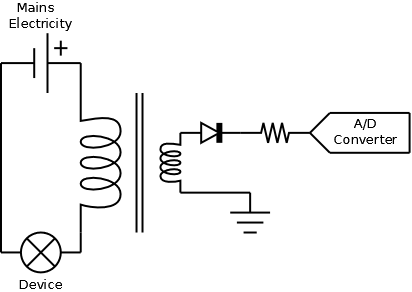
\includegraphics[scale=0.3]{Hardware/images/MeasureCircuit.png}

\section{Potential Problems}

% A list of potentional programs along with suggestions
%  on ways to work around them. Elaborate on why the problem
%  exists

\section{Sub-modules 1}

% This is a second section of modules,
%  and should consists of this module broken 
%  down further into components. This would
%  be where you expand on any component of the circuit
%  if that needs to be done